\section{Die Benutzerschnittstelle}
	In diesem Abschnitt dieses Kapitels wird auf die Implementierung der Benutzerschnittstelle eingegangen. Wie schon bereits im SRS erwähnt handelt es sich bei der Benutzerschnittstelle um die grafische Oberfläche der Android App. 
	
	\subsection{Grafische Oberfläche mit Unity}
		Die grafische Oberfläche, zu englisch User Interface (UI), wird mit Unity's zur Verfügung gestelltem UI System implementiert. Der Canvas, zu deutsch Leinwand, stellt dabei die Elternkomponente dar. Dieser enthält alle UI Elemente. Der Canvas verwendet dabei das EventSystem Objekt von Unity. Das Event System  ist eine Möglichkeit, Events auf Objekte in der Anwendung, basierend auf den Eingaben des Spielers, zu senden\footnote{Vgl. \url{https://docs.unity3d.com/Manual/EventSystem.html}}. Erst durch die Verwendung des Event Systems werden die Touchscreen-Eingaben an die App weitergegeben.
		
		All UI elements must be children of a GameObject that has a Canvas component attached. Zu den UI Elementen gehören: Unity bietet eine große Anzahl an vorgefertigten Standard Interaktionsobjekten. Dazu gehören zum Beispiel Buttons, ToggleButtons, Dropdown Listen, Input Felder und Scroll Views\footnote{Vgl. \url{https://docs.unity3d.com/Manual/UIInteractionComponents.html}}.
		
		Der Canvas hat in Unity drei Render-Modi\footnote{Vgl. \url{https://docs.unity3d.com/Manual/UICanvas.html}}. Je nachdem welcher Modus ausgewählt wurde, wird die grafische Oberfläche anders in das Spiel integriert.
		
		\subsubsection{Screen Space - Overlay}
			This render mode places UI elements on the screen rendered on top of the scene. If the screen is resized or changes resolution, the Canvas will automatically change size to match this.
			
			In this mode, the Canvas is scaled to fit the screen and then rendered directly without reference to the scene or a camera (the UI will be rendered even if there is no camera in the scene at all). If the screen’s size or resolution are changed then the UI will automatically rescale to fit. The UI will be drawn over any other graphics such as the camera view.
		
		\subsubsection{Screen Space - Camera}
			This is similar to Screen Space - Overlay, but in this render mode the Canvas is placed a given distance in front of a specified Camera. The UI elements are rendered by this camera, which means that the Camera settings affect the appearance of the UI. If the Camera is set to Perspective, the UI elements will be rendered with perspective, and the amount of perspective distortion can be controlled by the Camera Field of View. If the screen is resized, changes resolution, or the camera frustum changes, the Canvas will automatically change size to match as well.
			
			In this mode, the Canvas is rendered as if it were drawn on a plane object some distance in front of a given camera. The onscreen size of the UI does not vary with the distance since it is always rescaled to fit exactly within the camera frustum. If the screen’s size or resolution or the camera frustum are changed then the UI will automatically rescale to fit. Any 3D objects in the scene that are closer to the camera than the UI plane will be rendered in front of the UI, while objects behind the plane will be obscured.
		
		\subsubsection{World Space}
			In this render mode, the Canvas will behave as any other object in the scene. The size of the Canvas can be set manually using its Rect Transform, and UI elements will render in front of or behind other objects in the scene based on 3D placement. This is useful for UIs that are meant to be a part of the world. This is also known as a “diegetic interface”.
			
			This mode renders the UI as if it were a plane object in the scene. Unlike Screen Space - Camera mode, however, the plane need not face the camera and can be oriented however you like. The size of the Canvas can be set using its Rect Transform but its onscreen size will depend on the viewing angle and distance of the camera. Other scene objects can pass behind, through or in front of the Canvas.
			
	\subsection{Die Umsetzung}	
		Um die ergonomie zu erhöhen kann der linke joystick i einem festgelegten bereich überall angelegt werden
		
		Da es sich um KOmponenten handelt die immer da sein müssen wurde sich für das normale UI Screen Space - OVerlay ausgewählt
		
		\begin{figure}[htbp]
			\centering 
			\label{umlControl}
			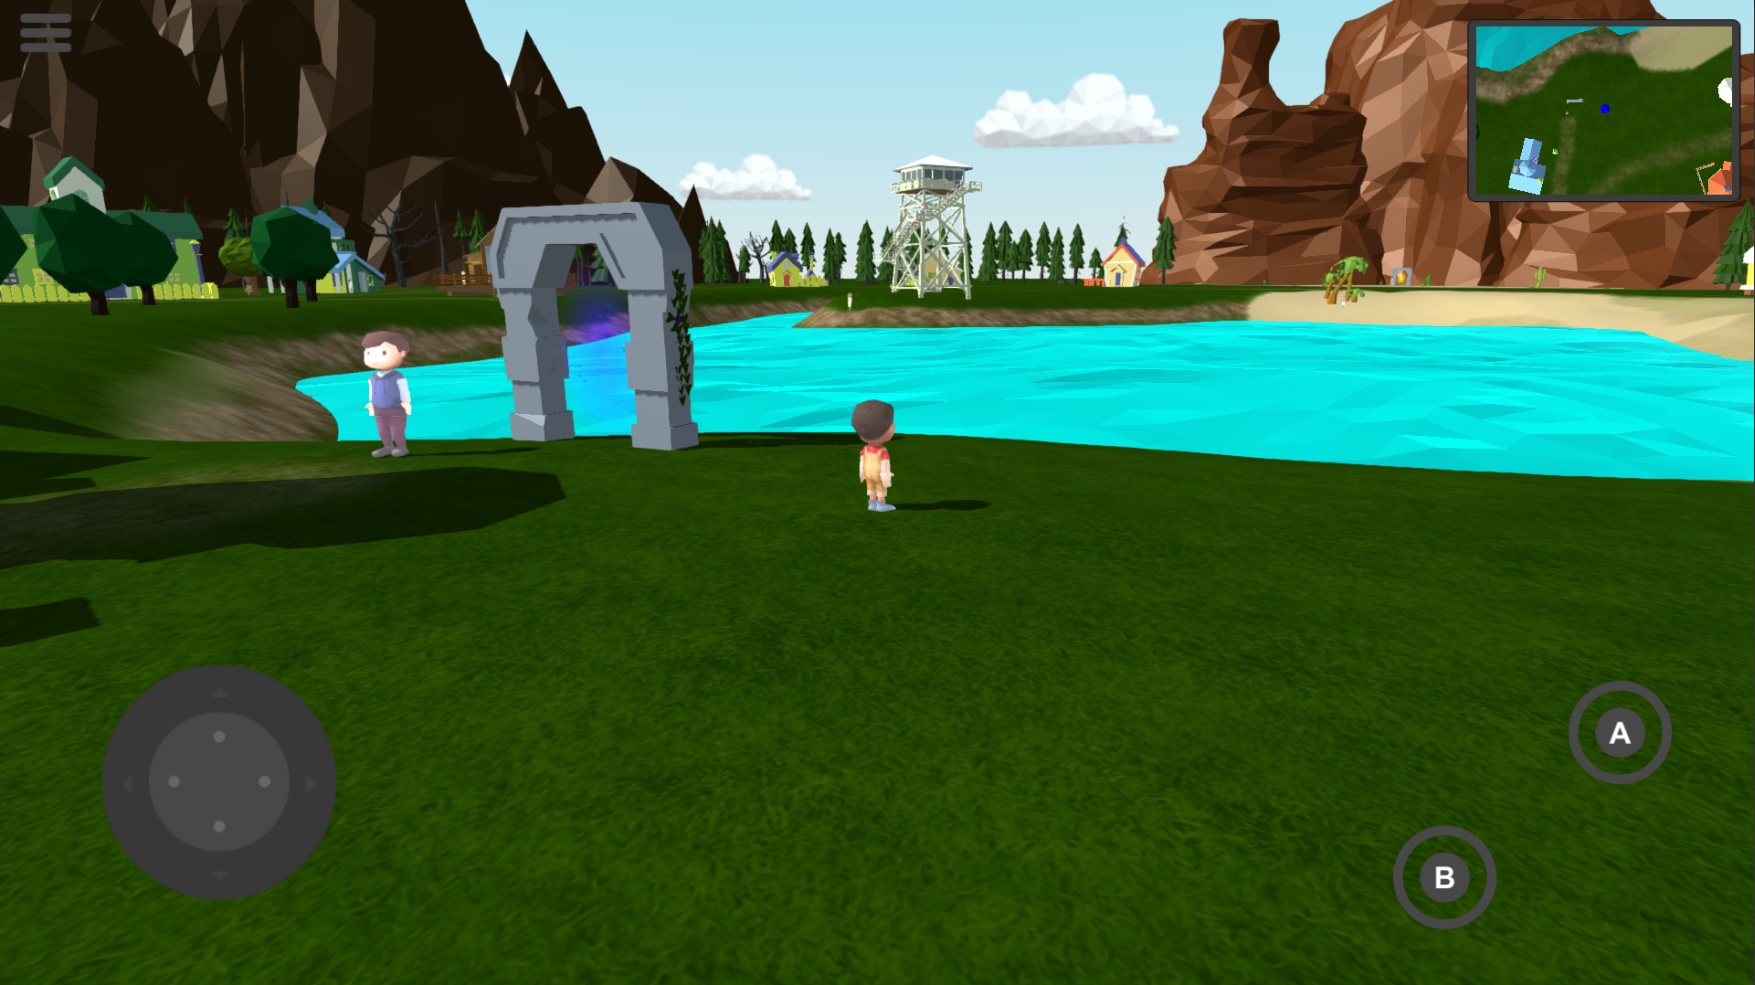
\includegraphics[width=13cm]{pics/alwaysOnUI.png}
			\caption{User Interface: Head-Up Display}
		\end{figure}
	
		\begin{figure}[htbp]
			\centering 
			\label{umlControl}
			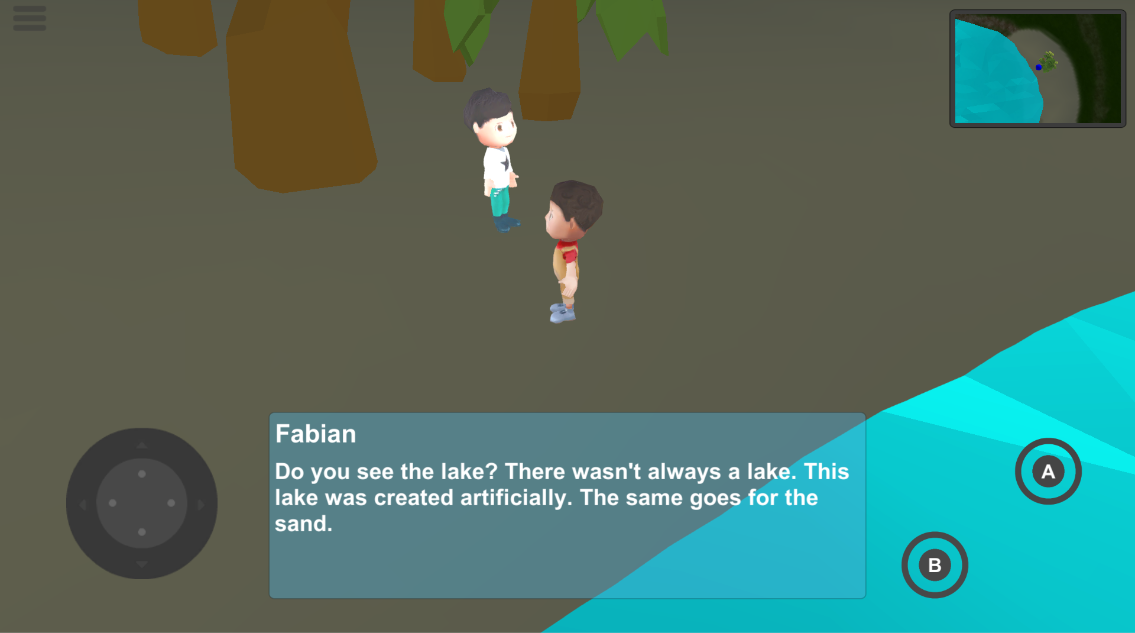
\includegraphics[width=13cm]{pics/communicationUI.png}
			\caption{User Interface: Aktive Kommunikation mit einem Non-Player Charakter}
		\end{figure}

		\begin{figure}[htbp]
			\centering 
			\label{umlControl}
			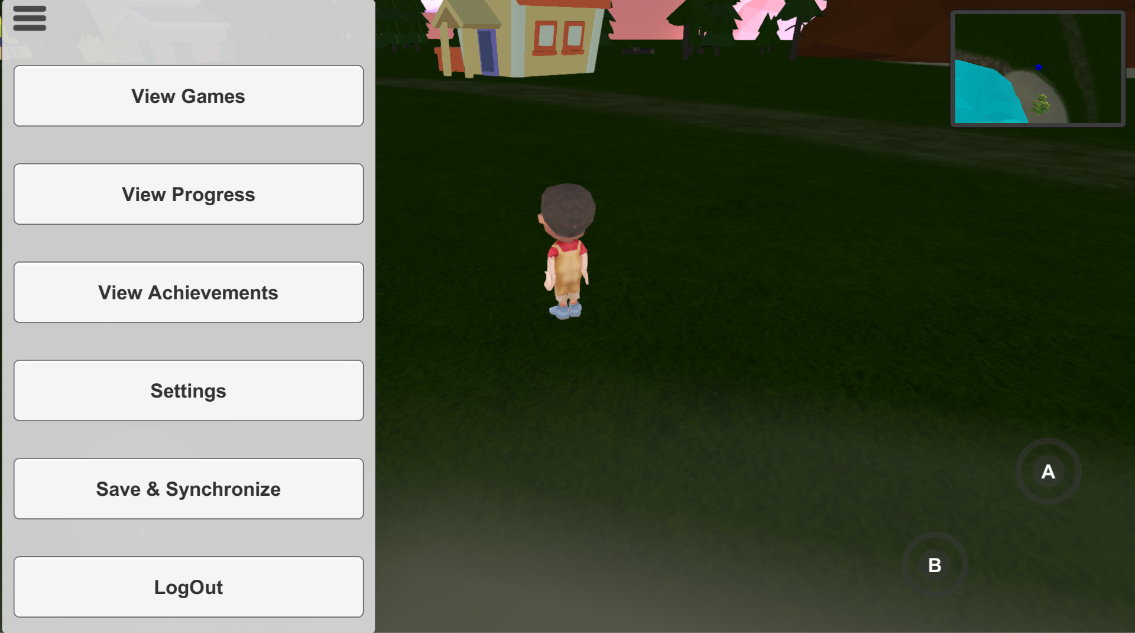
\includegraphics[width=13cm]{pics/menuUI.png}
			\caption{User Interface: Offenes Menu}
		\end{figure}
		
		\begin{figure}[htbp]
			\centering 
			\label{umlControl}
			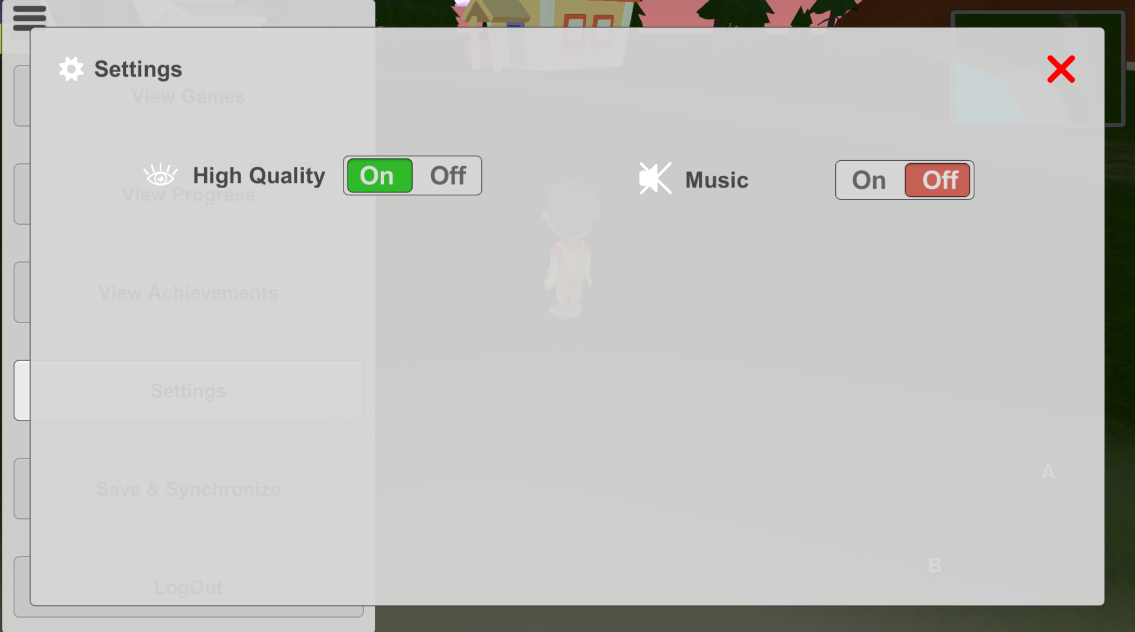
\includegraphics[width=13cm]{pics/settingsUI.png}
			\caption{User Interface: Einstellungen Fenster}
		\end{figure}

		\begin{figure}[htbp]
			\centering 
			\label{umlControl}
			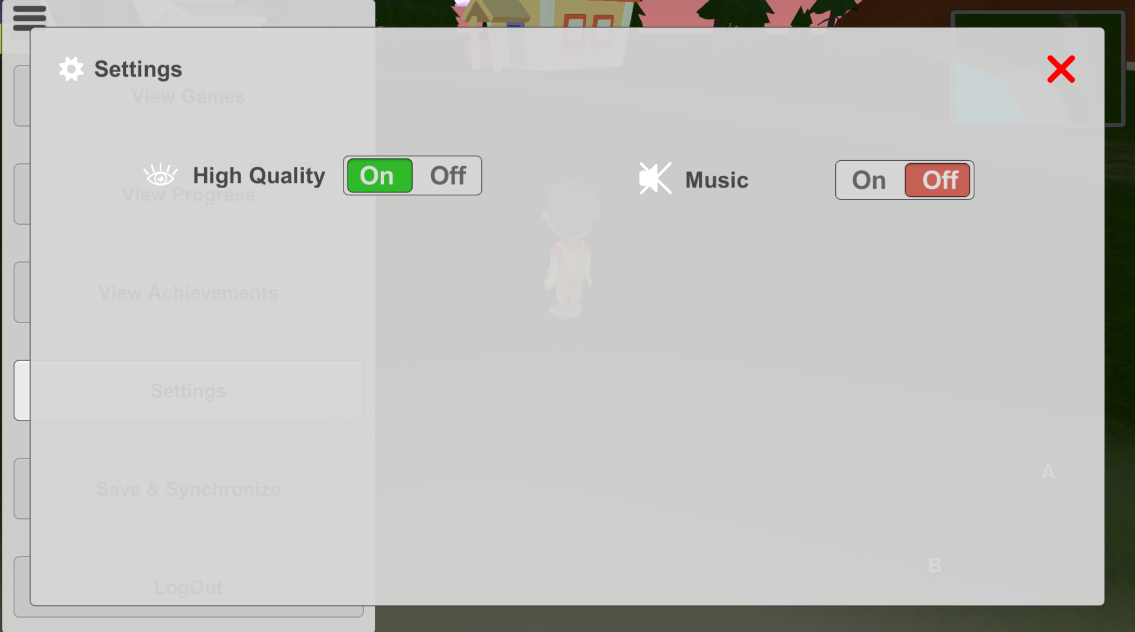
\includegraphics[width=13cm]{pics/settingsUI.png}
			\caption{User Interface: Registrierung}
		\end{figure}
	
		Dialogebene max. 1, es öffnet sich max immer ein Dialog dieser dient zum Abbrechen, warnt vor bevorstehenden Aktionen
	
	\subsection{Usability Test}
		Usability TEst faken? Kinder + Jugendliche --> Katalog mit Bewertung
		Summativer TEst: Nach der Entwicklung, fertiges Produkt vor Auslieferung umfangreiche Studie
	
		Benutzerprofiele, Szenarien, Umfang, Zeitraum (3 Tage) 
	
		TEstutensilien: Prerelease version der APp und eigene Software
		Testart: Remotetest (vor und nachteile zu anderen)